\documentclass{report}
\usepackage[T1]{fontenc}
\usepackage[utf8]{inputenc}
\usepackage[english]{babel}
\usepackage{graphicx}
\usepackage[hidelinks]{hyperref}
\usepackage{fancyhdr}
\pagestyle{fancy}
\lhead{\textbf{System and device programming}}
\rhead{Laboratory 5}
\lfoot{Enrico Franco}
\rfoot{Politecnico di Torino}
\author{Enrico Franco}
\title{System and Device Programming \\
	Laboratory 5 - Exercise 2}
\begin{document}
\section*{Exercise 2}
The GDT and the IDT are descriptor tables. They are arrays of flags and bit values describing the operation of either the segmentation system, or the interrupt vector table.

\subsection*{The Global Descriptor Table}
GRUB sets a standard GDT but its location is not known, so it may be accidentally overwritten, causing a series of faults and a reset. In the x86 architecture, there are six segmentation registers and each holds an offset into the GDT.

\subsubsection*{\texttt{descriptor\_tables.h}}
\texttt{descriptor\_tables.h} defines the interface for initializing the GDT and IDT and needed structures.
A GTD entry looks like:

\begin{figure}[hbtp]
\centering
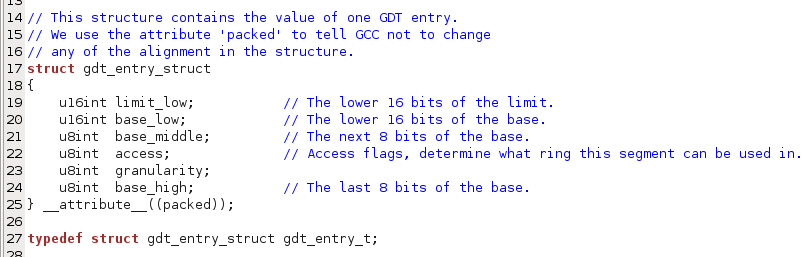
\includegraphics[scale=0.4]{images/es02/gdt_entry.png}
\caption{GDT entry}
\end{figure}

The format of the \emph{access byte} is given from
\begin{center}
\begin{tabular}{|c|c|c|c|}
\hline 
P & DPL & DT & Type \\ 
\hline 
\end{tabular}
\end{center}
where:
\begin{itemize}
\item \textbf{P} (1 bit) - Is segment present? (1 = Yes)
\item \textbf{DPL} (2 bit) - Descriptor privilege level
\item \textbf{DT} (1 bit) - Descriptor type
\item \textbf{Type} (4 bit) - Segment type (code or data)
\end{itemize}
and the format of the \emph{granularity byte} is given from
\begin{center}
\begin{tabular}{|c|c|c|c|c|}
\hline 
G & D & 0 & A & Segment lenght \\ 
\hline 
\end{tabular}
\end{center}
where:
\begin{itemize}
\item \textbf{G} (1 bit) - Granularity (0 = 1 byte, 1 = 1 Kbyte)
\item \textbf{D} (1 bit) - Operand size (0 = 16 bit, 1 = 32 bit)
\item \textbf{0} (1 bit) - Should be always zero
\item \textbf{A} (1 bit) - Available for system use, always zero
\item \textbf{Segment lenght} (4 bit)
\end{itemize}

In order to inform the processor where to find GDT, it is needed to give it the address of a special pointer structure, where the \texttt{base} represents the address of the first entry in the GDT and the \texttt{limit} represents the last valid address in the table, i.e.\@ the size of the table minus one. 

\begin{figure}[hbtp]
\centering
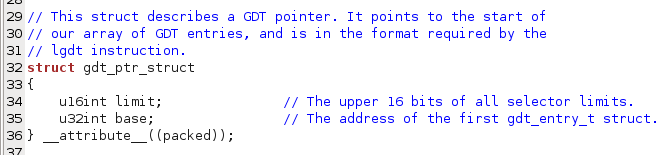
\includegraphics[scale=0.4]{images/es02/gdt_ptr.png}
\caption{GDT pointer}
\end{figure}

Header file \texttt{descriptor\_tables.h} defines also a prototype, permitting the initialization of tables.

\begin{figure}[hbtp]
\centering
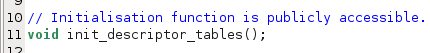
\includegraphics[scale=0.4]{images/es02/gdt_init.png}
\caption{GDT init prototype}
\end{figure}

\subsubsection*{\texttt{descriptor\_tables.c}}
\texttt{descriptor\_tables.c} initializes the GDT and IDT and defines the default ISR and IRQ handlers.

In \texttt{descriptor\_tables.c}, we have a few declarations. \texttt{gdt\_flush} function, defined in an ASM file, loads GDT pointer. 

\texttt{init\_descriptor\_tables()}, as shown in figure~\ref{descriptor_tables_init}, calls some functions to initialize all the interrupt service routines, the GDT and the IDT.

\begin{figure}[hbtp]
\centering
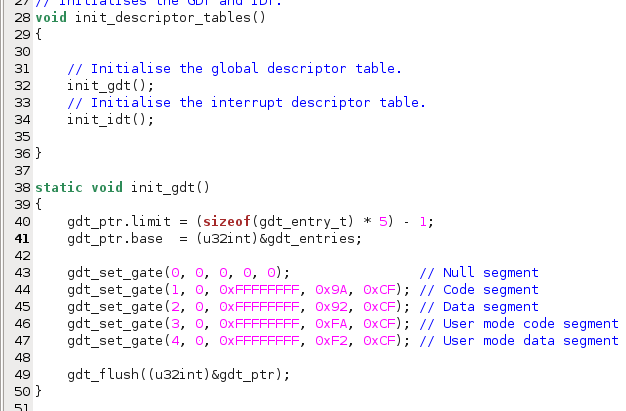
\includegraphics[scale=0.4]{images/es02/descriptor_tables_init.png}
\caption{GDT initialization}
\label{descriptor_tables_init}
\end{figure}

Analyzing that code, \texttt{init\_gdt} initially sets up the gdt pointer structure. The \texttt{limit} is the size of each gdt entry * 5 because it is needed to represent some descriptors: code and data segment descriptor for the kernel, code and data segment descriptors for user mode, and a null entry. \texttt{gdt\_init} then sets up the 5 descriptors, by calling \texttt{gdt\_set\_gate}.

Finally, the ASM function writes the GDT pointer.
\texttt{gdt.s} contains global descriptor table and interrupt descriptor table setup code.

\begin{figure}[hbtp]
\centering
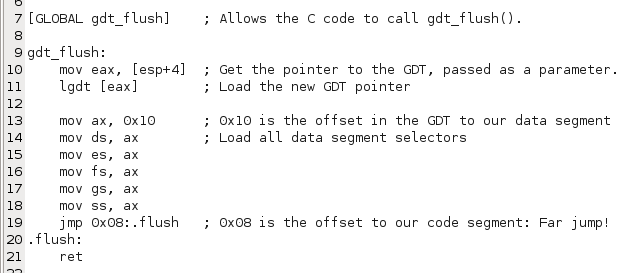
\includegraphics[scale=0.4]{images/es02/gdt_flush.png}
\caption{gdt\_flush}
\label{gdt_flush}
\end{figure}

This function, shown in figure~\ref{gdt_flush}, takes the first parameter passed to it (in \texttt{esp+4}), loads the value it points to into the GDT and loads the segment selectors for the data and code segments. Each GDT entry is 8 bytes: the kernel code descriptor is the second segment and the kernel data descriptor is the third.

\newpage
\subsection*{The Interrupt Descriptor Table}
The Interrupt Descriptor Table informs the processor where to find handlers for each interrupt. It is just an array of entries, each one corresponding to an interrupt number. If an interrupt occurs and there is no entry for it (even a NULL entry is fine), the processor will reset. 

The processor may need to signal the kernel informing that something major may have happened. To do this, it uses the first 32 interrupts, which are the most important and all of these must be mapped, otherwise the CPU will reset. 

\subsubsection*{\texttt{descriptor\_tables.h}}
Some definitions have to be added in file \texttt{descriptor\_tables.h}.
In a similar way to the GDT entry and pointer, IDT entry and pointer have to be defined.

\begin{figure}[hbtp]
\centering
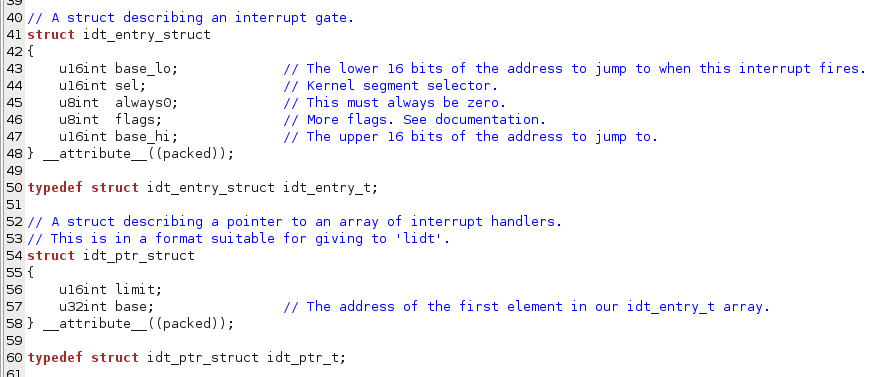
\includegraphics[scale=0.36]{images/es02/idt_definitions.png}
\caption{IDT entry and pointer}
\end{figure}

The flags field format is given from 
\begin{center}
\begin{tabular}{|c|c|c|}
\hline 
P & DL & Lower 5-bits \\ 
\hline 
\end{tabular}
\end{center}
where:
\begin{itemize}
\item \textbf{P} (1 bit) - Is segment present? (1 = Yes)
\item \textbf{DPL} (1 bit) - Descriptor privilege level
\item \textbf{Lower 5-bits} (5 bit) - Should be always 14 in decimal. Any descriptor with this bit clear will cause a "Interrupt Not Handled" exception
\end{itemize}

\subsubsection*{\texttt{descriptor\_tables.c}}
Similar code is needed to initialize the IDT as shown in figure~\ref{idt_init} and in \texttt{gdt.s} to allow the code C to call \texttt{idt\_flush()} as shown in figure~\ref{idt_flush}.
\begin{figure}[hbtp]
\centering
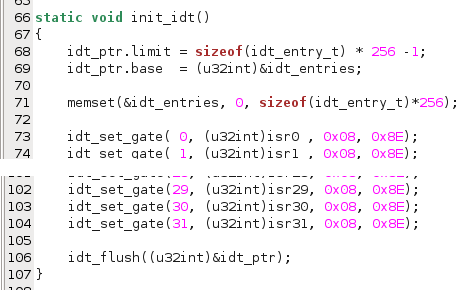
\includegraphics[scale=0.5]{images/es02/idt_init.png}
\caption{IDT initialization}
\label{idt_init}
\end{figure}

\begin{figure}[hbtp]
\centering
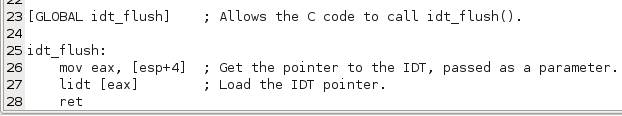
\includegraphics[scale=0.4]{images/es02/idt_flush.png}
\caption{idt\_flush}
\label{idt_flush}
\end{figure}

\subsubsection*{\texttt{interrupt.s}}
\texttt{interrupt.s} contains interrupt service routine wrappers.

At this point, the CPU knows where to find interrupt handlers, but they are not written yet. When the processor receives an interrupt, it saves the contents of the essential registers to the stack. Then, it finds the interrupt handler location from the IDT and jumps to it.

It is not possible to have one common handler, instead different ones must be defined for each interrupt to handle. In fact handlers just push the interrupt number (hardcoded in the ASM) onto the stack, and call a common handler function. Unfortunately, some interrupts also push an error code onto the stack. Thus, for those that don't push an error code, dummy one is pushed, so the stack is the same.

Using NASM's macro facility is possible to write a single ``general'' routine, as shown in figure~\ref{isr_macros} and make a stub handler function. In particular, Intel manual shows that only interrupts 8, and from 10 to 14 inclusive push error codes onto the stack; all the others require dummy error codes.

\begin{figure}[hbtp]
\centering
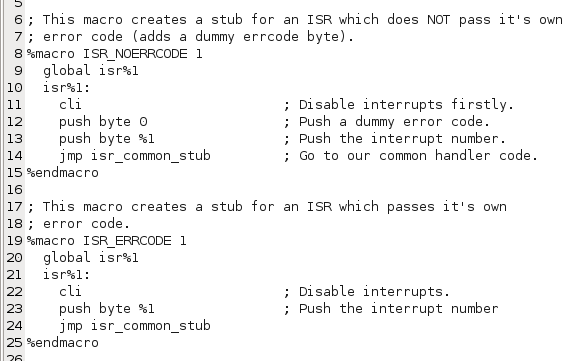
\includegraphics[scale=0.4]{images/es02/isr_macros.png}
\caption{ISR macros}
\label{isr_macros}
\end{figure}

An ASM common handler function and a higher-level C handler function have to be created.

The ASM common handler is shown in figure~\ref{isr_handler}. First, it pushes all the register and the data segment selector on the stack. It sets sets all the segment registers to the kernel data selector and it calls a higher-level interrupt handler \texttt{isr\_handler}. When an interrupt fires, the processor automatically pushes information about the processor state onto the stack. The \texttt{iret} instruction is specifically designed to return from an interrupt. It pops these values off the stack and returns the processor to the state it was in originally. 

\begin{figure}[hbtp]
\centering
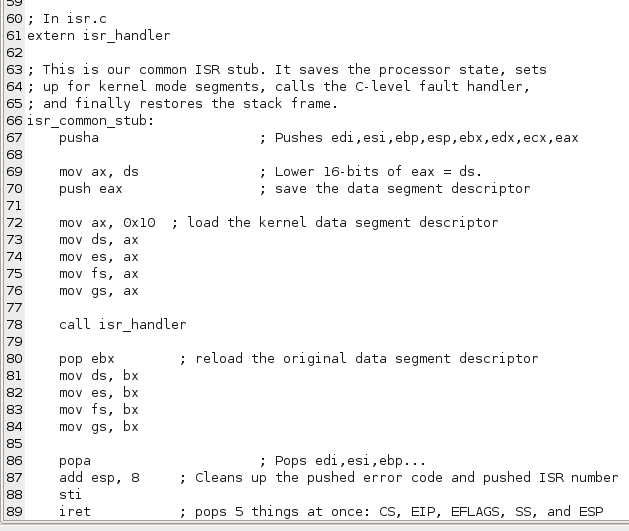
\includegraphics[scale=0.4]{images/es02/isr_handler.png}
\caption{ISR handler}
\label{isr_handler}
\end{figure}

\subsubsection*{\texttt{isr.c}}
\texttt{isr.c} contains high level interrupt service routines and interrupt request handlers.

The interrupt handler prints a message on the screen, including the interrupt number it handled. It uses a structure \texttt{registers\_t}, which is a representation of all the registers we pushed, defined in \texttt{isr.h}.

\begin{figure}[hbtp]
\centering
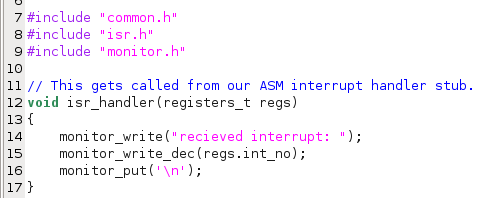
\includegraphics[scale=0.4]{images/es02/isr_c.png}
\caption{isr.c}
\end{figure}

\subsubsection*{\texttt{isr.h}}
\texttt{isr.h} defines interface and structures for high level interrupt service routines.

\begin{figure}[hbtp]
\centering
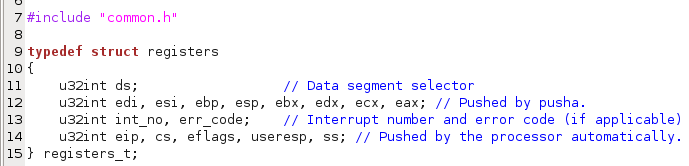
\includegraphics[scale=0.4]{images/es02/isr_h.png}
\caption{isr.h}
\end{figure}

\subsubsection*{Testing}
In order to test it, \texttt{main()} function must contain some interrupt requests as shown in figure~\ref{isr_main}.

\begin{figure}[hbtp]
\centering
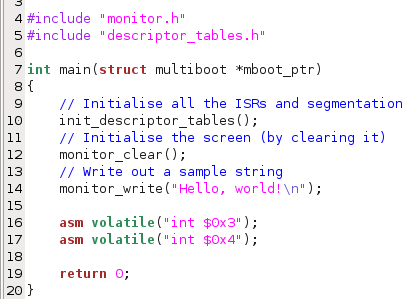
\includegraphics[scale=0.4]{images/es02/main.png}
\caption{isr.c}
\label{isr_main}
\end{figure}

In figure~\ref{isr_single_interrupt} only the first interrupt has been received, while figure~\ref{isr_final_state} shows the final state, i.e.\@ both interrupt has been received.

\begin{figure}[hbtp]
\centering
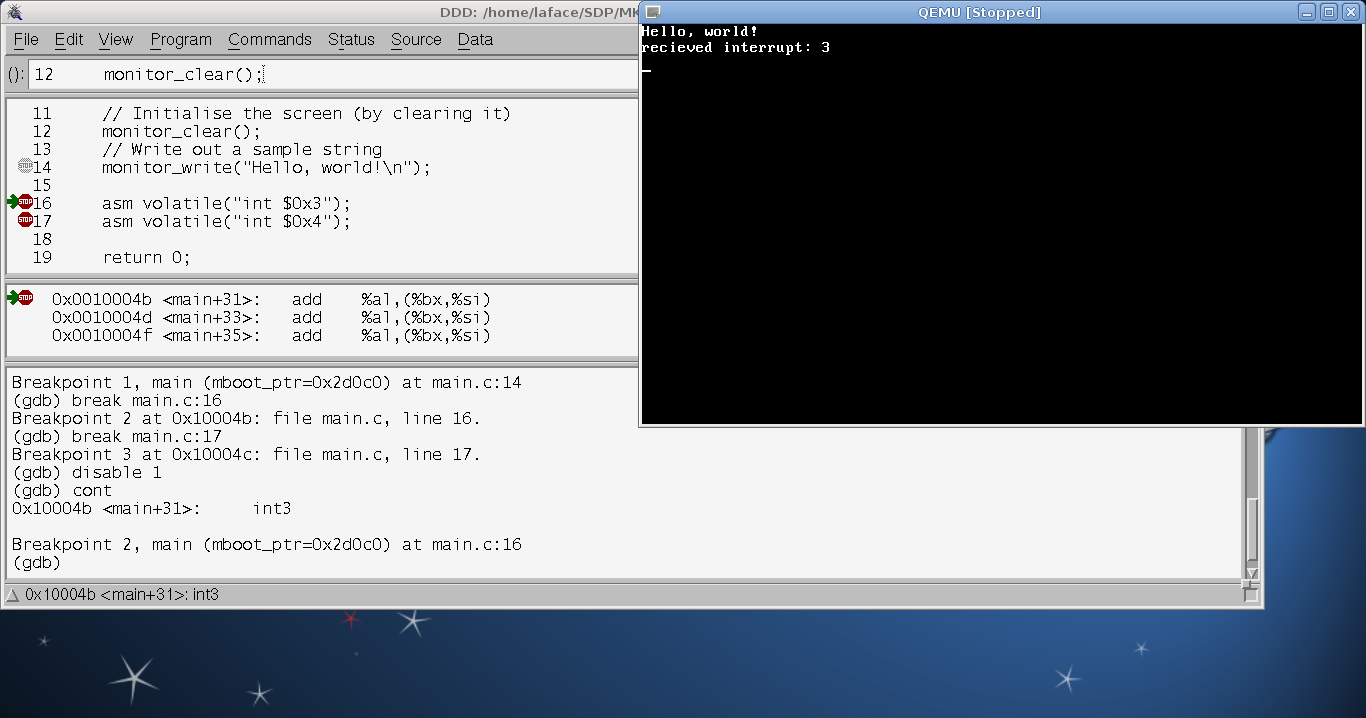
\includegraphics[scale=0.25]{images/es02/isr_single_interrupt.png}
\caption{Single interrupt received}
\label{isr_single_interrupt}
\end{figure}

\begin{figure}[hbtp]
\centering
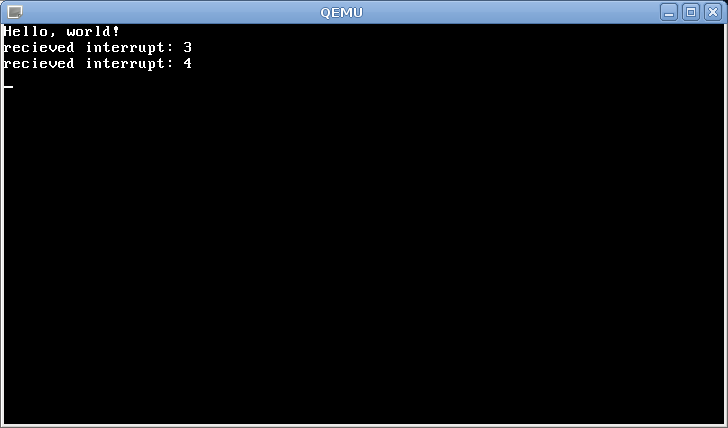
\includegraphics[scale=0.4]{images/es02/isr_final_state.png}
\caption{Interrupts received}
\label{isr_final_state}
\end{figure}

\end{document}